
%(BEGIN_QUESTION)
% Copyright 2008, Tony R. Kuphaldt, released under the Creative Commons Attribution License (v 1.0)
% This means you may do almost anything with this work of mine, so long as you give me proper credit

Determine what will happen to all voltage drops in this circuit if the resistance of resistor $R_3$ happens to increase:

$$\includegraphics[width=15.5cm]{i02909x01.eps}$$

\begin{itemize}
\item{} $V_{R1}$ = ({\it increase}, {\it decrease}, or {\it stay the same})
\vskip 10pt
\item{} $V_{R2}$ = ({\it increase}, {\it decrease}, or {\it stay the same})
\vskip 10pt
\item{} $V_{R3}$ = ({\it increase}, {\it decrease}, or {\it stay the same})
\vskip 10pt
\item{} $V_{R4}$ = ({\it increase}, {\it decrease}, or {\it stay the same})
\end{itemize}

\vfil 

\underbar{file i02909}
\eject
%(END_QUESTION)





%(BEGIN_ANSWER)

This is a graded question -- no answers or hints given!

%(END_ANSWER)





%(BEGIN_NOTES)

\begin{itemize}
\item{} $V_{R1}$ = {\bf decrease}
\vskip 10pt
\item{} $V_{R2}$ = {\bf decrease}
\vskip 10pt
\item{} $V_{R3}$ = {\bf increase}
\vskip 10pt
\item{} $V_{R4}$ = {\bf decrease}
\end{itemize}

%INDEX% Electronics review: qualitative analysis of DC series resistor circuit

%(END_NOTES)


